\section{アンカーの発話区間の音声認識実験}

\subsection{実験方法}

\subsection{音響モデルの仕様}
本実験で用いたDNN-HMM音響モデルの仕様を表\ref{table:acoustic_model_detail}に示す。この仕様に関しては小島らの研究[10]で使用されたもので、状態数は3000、音響特徴の次元数は39次元(表\ref{acoustic_model_feature})、隠れ層の数は6層、各層における繰り返し学習数は5回、隠れ層のノード数は1024とした。以下に、DNNを用いた際の学習の手順を示す。

\begin{table}[H]
  \begin{center}
    \caption{音響モデルの仕様 \label{table:acoustic_model_detail}}
    \begin{tabular}{|c|c|c|} \hline
     状態数  & 使用した音素 & 混合数 \\ \hline
     3,000  & 27 & 16 \\ \hline
    \end{tabular}
  \end{center}
\end{table}

\begin{table}[H]
  \begin{center}
    \caption{使用する音響特徴パラメータ \label{acoustic_model_feature}}
    \begin{tabular}{|c||c|} \hline
      特徴量 & 次元数\\ \hline
      MFCC & 12  \\ \hline
      POW & 1  \\ \hline
      $\Delta$MFCC & 12 \\ \hline
      $\Delta$POW & 1 \\ \hline
      $\Delta\Delta$MFCC & 12 \\ \hline
      $\Delta\Delta$POW & 1 \\ \hline
      計 & 39 \\ \hline
    \end{tabular}
  \end{center}
\end{table}

\vspace{0.2in}\noindent{\textbf{\underline{構築手順}}}\par
DNNを用いた音響モデルの構築や、この音響モデルを用いた音声認識に必要な学習テキストや言語モデルを作成する為にKaldiツールキットを用いた[11]。このツールキットの大きな流れを図\ref{fig:flow_train_dnn}に示す。まず学習や評価に必要なデータを用意し、言語モデルと単語辞書のWeighted Finite State Transducer (WFST)を作成する。WFSTとは重み付き有限トランスデューサといい、状態遷移機械モデル有限オートマトンの一種である。次に音声データから特徴量を抽出したデータを準備し、このデータと書き起こしを用いてGMM-HMMによる音響モデルのWFSTを作成する。これらのWFSTを、合成等を行ない1つのWFSTとする。このWFSTを用いて音声認識を行ない、学習データのアライメント(フレームごとの音素情報)をとる。このアライメントを用いてDNNを用いた音響モデルの学習(プレトレーニングと微調整)を行ない、最終的な音声認識を行なう。

\begin{figure}[H]
  \begin{center}
    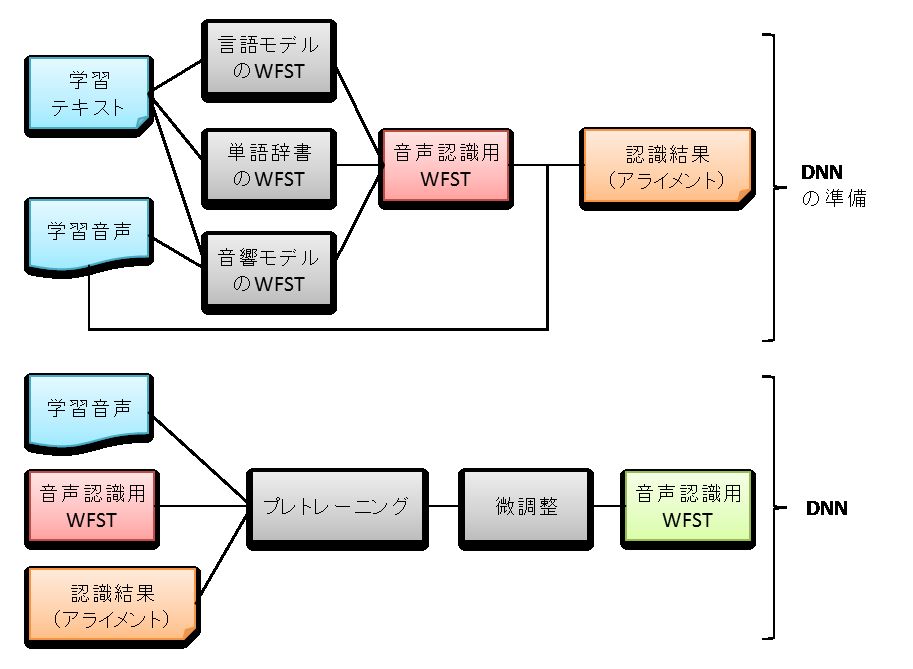
\includegraphics{./figure/flow_train_dnn.eps}
  \end{center}
  \caption{DNNを用いる際の学習の流れ \label{fig:flow_train_dnn}}
\end{figure}

\vspace{0.2in}\noindent{\textbf{\underline{使用コーパス}}}\par
音声認識は統計的モデルを用いるため、大量の音声・言語素材が必要である。本研究では2004年、国立国語研究所・情報通信研究機構・東京工業大学が共同開発した「日本語話し言葉コーパス」(Corpus of Spontaneous Japanese : CSJ)を使用する。このCSJは日本語の自発音声を大量に集めて多くの研究用情報を付加した話し言葉研究用データベースである。コーパスとは様々な研究機関において共通に利用可能な大量のデータのことである。全体で約660時間の自発音声(語数にして約700万個)が格納されている。\par
CSJに収録されている音声の種類と分量を表\ref{table:detail_csj}に示す。学会講演は、国内の様々な学会でライブ録音された研究発表音声である。収録された学会は、工学ないし自然科学系が3学会、621ファイル、人文科学系が4学会、187ファイル、社会科学系が2学会、169ファイルであり、理工学系の学会での話者は男性の大学院生であることが多いため、学会講演の話者は年齢と性別に偏りがある。講演時間は、大部分が12分から25分程度の長さであるが、なかには1時間を超える招待講演の類も含まれている。模擬講演は、人材派遣会社によって選定された一般話者による日常話題についての「スピーチ」である。模擬講演の話者は、性別と年齢がほぼ均等に分布されている。話者は三つの大まかなテーマを与えられ、それぞれについて平均12分程度のスピーチを行なった。\par

\begin{table}[htb]
  \begin{center}
    \caption{CSJの音声の種類と分量 \label{table:detail_csj}}
    \begin{tabular}{|c||c|c|c|c|} \hline
      音声の種類 & 話者数 & ファイル数 & 独話・対話 & 時間数\\ \hline
      学会講演 & 838 & 1007 & 独話 & 299.5 \\ \hline
      模擬講演 & 580 & 1699 & 独話 & 324.1 \\ \hline
      朗読音声 & 244 & 491 & 独話 & 14.1 \\ \hline
      インタビュー話者による模擬講演 & 16 & 16 & 独話 & 3.4 \\ \hline
      学会講演インタビュー & 10 & 10 & 対話 & 2.1 \\ \hline
      模擬講演インタビュー & 16 & 16 & 対話 & 3.4 \\ \hline
      課題志向対話 & 16 & 16 & 対話 & 3.1 \\ \hline
      自由対話 & 16 & 16 & 対話 & 3.6 \\ \hline
      再朗読 & 16 & 16 & 独話 & 5.5\\ \hline
    \end{tabular}
  \end{center}
\end{table}


\vspace{0.2in}\noindent{\textbf{\underline{使用した音素}}}\par
本研究で使用した音素27個を表\ref{fig:used_onso}に示す。また、その音素をもとに記したカナ音素対応表を表\ref{fig:kana_onso}に示す

\begin{table}[H]
  \begin{center}
    \caption{使用した音素 \label{fig:used_onso}}
    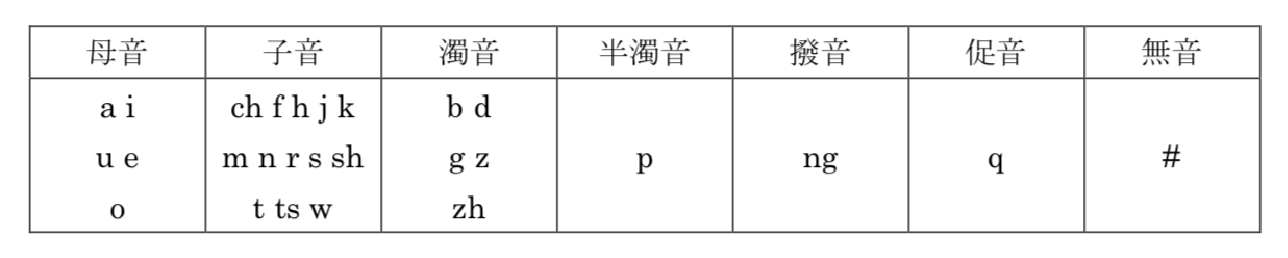
\includegraphics[scale=0.7]{./figure/used_onso.eps}
  \end{center}
  
\end{table}

\begin{table}[H]
  \begin{center}
    \caption{カナ音素対応表 \label{fig:kana_onso}}
    \includegraphics[scale=0.7]{./figure/kana_onso.eps}
  \end{center}
  
\end{table}

\vspace{0.2in}\noindent{\textbf{\underline{木構造話者クラスタ}}}\par
先行研究[2][3]では、話者の音響特徴、話者特徴ごとに作成した木構造話者クラスタ、音響モデルを作成することで音声認識精度の向上を確認したため、本研究でも使用する。このクラスタは、母音の定常状態であるHMMの中央の状態の平均と分散を用いたBhattacharyya距離によるk-means法によって作成した。クラスタの個数は、最上位のクラスタを2分割し、作成された2つのクラスタをさらに2分割した計7つのクラスタを使用する。


\subsection{言語モデル・単語辞書の仕様}
言語モデルはトライグラムモデルを構築した。以下、使用した学習テキストを説明する。

\vspace{0.2in}\noindent{\textbf{\underline{CSJ}}}\par
CSJには書き起こしテキストも提供されており、その一部の例を図\ref{fig:kakiokosi}に示す。書き起こしテキストは主に情報部と発話部に区別される。情報部では発話IDや時間情報等を、発話部では発話内容を「&」の左側に基本形、右側に発音形という形式で記している。発話形はカタカナを用いて実際に発音された音声を忠実に表記したものである。発音の怠けや言い間違い等を書き取れる範囲で忠実に記録している。本研究では、音響モデル構築の際には主に発話部の発音形を用い、このカタカナ表記を音素列に変換し、ラベルファイルとして定義する。
\begin{figure}[H]
  \begin{center}
    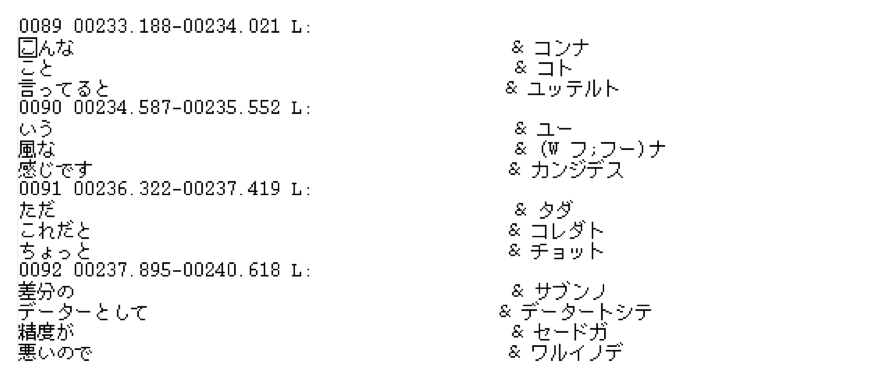
\includegraphics{./figure/kakiokosi.eps}
  \end{center}
  \caption{書き起こしテキストの例 \label{fig:kakiokosi}}
\end{figure}

本研究ではこのCSJをベースに学習テキストを構成する。使用するデータは977講演分のテキストで、約14MBである。

\vspace{0.2in}\noindent{\textbf{\underline{拡張したコーパスによる学習テキスト}}}\par
この学習テキストは江頭らによる、学術講演の書き起こしと新聞記事に拡張されるテキストとして参加者名の入ったテキスト、Webから収集してきたテキスト、そして対話コーパスから作成される対話テキストを追加した未知語の減少に着目した学習テキストである。この学習テキストは会議中に参加者の名前を呼ぶことが多い、会議は対話形式であるなどの会議の特徴を考慮した学習テキストである。テキストサイズは約100MBである。以降本論文では、このテキストを拡張したコーパスによる学習テキストと呼ぶ。

\vspace{0.2in}\noindent{\textbf{\underline{拡張したコーパスによる学習テキスト}}}\par
この学習テキストは荒井らによる、会議における発話行為に着目して作成された学習テキストである。学術講演の書き起こしと新聞記事に対話表現に近い特徴を持っていると考えられるQ&Aサイトから収集したテキストと対話コーパスを追加した学習テキストである。テキストサイズは約44MBである。以降本論文ではこのテキストを対話特化テキストと呼ぶ。


\subsection{評価方法}
本研究では評価尺度としては式\ref{calc:word_acc}で与えられる単語正解精度$Acc$(Word Accuracy)を用いる。ここで$W$は単語数、$S$(Substitution)は置換誤り、$D$(Deletion)は脱落誤り、$I$(Insertions)は挿入誤りの単語数を表わす。置換誤りとは、正解の単語が別の単語に誤認識された場合の誤りである。脱落誤りとは、単語があるべき部分に認識結果が何も出力されなかった場合の誤りである。挿入誤りは、本来単語がない部分に誤認識結果として単語が出力された場合の誤りである。

\begin{equation}
\label{calc:word_acc}
Acc=\frac{(W-S-D-I)}{W}
\end{equation}

          
評価は、正解ファイルと認識結果のファイルをDPマッチングを行なうことにより算出する。この正解ファイルは形態素解析した結果の形態素列によって作成したものである。
また、本研究ではアンカーの発話区間を対象とした音声認識を行うため、\ref{chapter:get_anchor}章で検出した発話区間より、アンカー以外の発話区間で認識された単語は全て挿入誤り、アンカーの発話として検出出来なかった発話区間の単語は全て削除誤りとして計算する。
\subsection{実験結果}
\subsection{考察}
